
% https://github.com/davidstutz/latex-resources/blob/master/tikz-gradient-descent/gradient-descent.tex
% \usepackage{tikz}
% \usepackage{tikz}
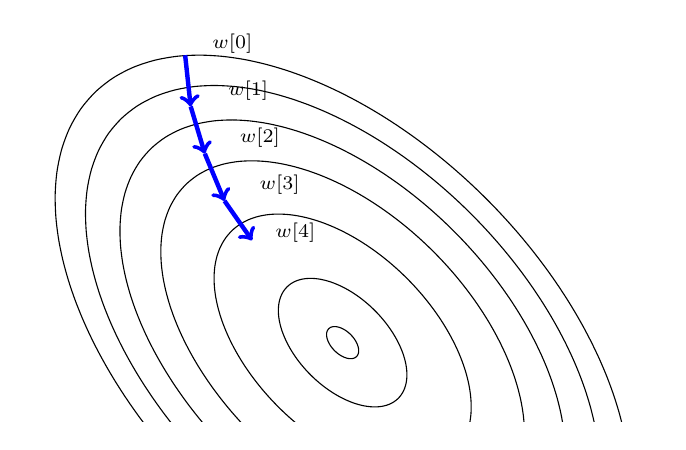
\begin{tikzpicture}[samples=100,smooth]
    \begin{scope}
        \clip(-4,-1) rectangle (4,4);
        \draw plot[domain=0:360] ({cos(\x)*sqrt(20/(sin(2*\x)+2))},{sin(\x)*sqrt(20/(sin(2*\x)+2))});
        \draw plot[domain=0:360] ({cos(\x)*sqrt(16/(sin(2*\x)+2))},{sin(\x)*sqrt(16/(sin(2*\x)+2))});
        \draw plot[domain=0:360] ({cos(\x)*sqrt(12/(sin(2*\x)+2))},{sin(\x)*sqrt(12/(sin(2*\x)+2))});
        \draw plot[domain=0:360] ({cos(\x)*sqrt(8/(sin(2*\x)+2))},{sin(\x)*sqrt(8/(sin(2*\x)+2))});
        \draw plot[domain=0:360] ({cos(\x)*sqrt(4/(sin(2*\x)+2))},{sin(\x)*sqrt(4/(sin(2*\x)+2))});
        \draw plot[domain=0:360] ({cos(\x)*sqrt(1/(sin(2*\x)+2))},{sin(\x)*sqrt(1/(sin(2*\x)+2))});
        \draw plot[domain=0:360] ({cos(\x)*sqrt(0.0625/(sin(2*\x)+2))},{sin(\x)*sqrt(0.0625/(sin(2*\x)+2))});

        \draw[->,blue,ultra thick] (-2,3.65) to (-1.93,3);
        \draw[->,blue,ultra thick] (-1.93,3) to (-1.75,2.4);
        \draw[->,blue,ultra thick] (-1.75,2.4) to (-1.5,1.8);
        \draw[->,blue,ultra thick] (-1.5,1.8) to (-1.15,1.3);

        \node at (-1.4,3.8){\scriptsize $w[0]$};
        \node at (-1.2,3.2){\scriptsize $w[1]$};
        \node at (-1.05,2.6){\scriptsize $w[2]$};
        \node at (-0.8,2){\scriptsize $w[3]$};
        \node at (-0.6,1.4){\scriptsize $w[4]$};
    \end{scope}
\end{tikzpicture}
